\documentclass[tikz,border=10pt]{standalone}
\usepackage{times}
\usepackage{amsmath,amssymb}
\usetikzlibrary{positioning,fit,arrows.meta,backgrounds,shapes.geometric,calc,shadows,decorations.pathreplacing,shapes}

\begin{document}
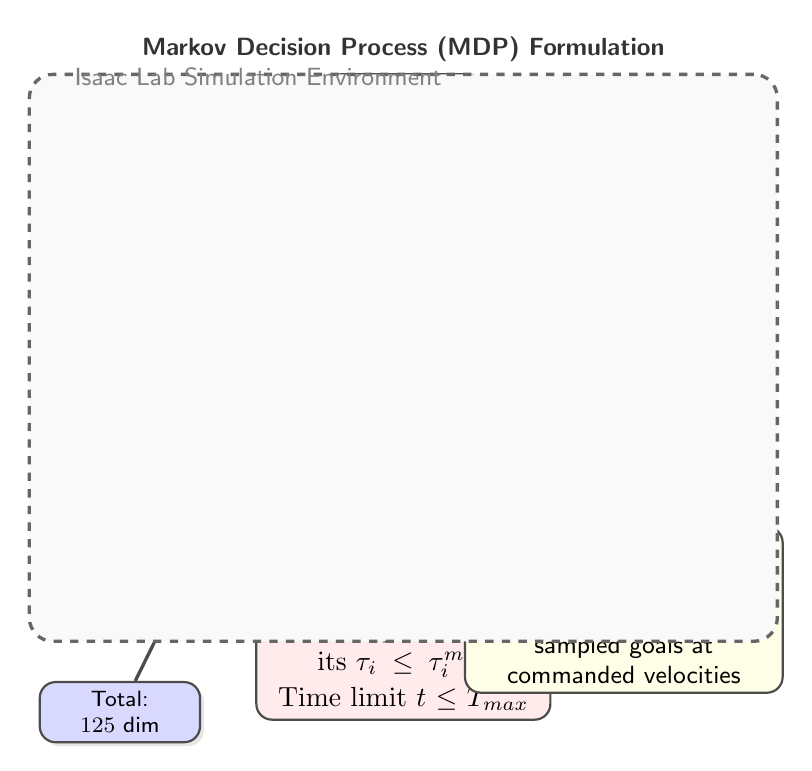
\begin{tikzpicture}[
    node distance=1.2cm and 1.8cm,
    box/.style={
        draw=black!70,
        rounded corners=2mm,
        fill=white,
        thick,
        font=\sffamily\footnotesize,
        text width=1.8cm,
        align=center,
        drop shadow={opacity=0.2, shadow xshift=0.05cm, shadow yshift=-0.05cm}
    },
    header/.style={
        font=\sffamily\bfseries\small,
        color=black!80
    },
    formula/.style={
        font=\ttfamily\tiny,
        color=black!60
    },
    arrow/.style={->, >=Stealth, thick, color=black!70},
    label/.style={font=\sffamily\tiny, color=black!60}
]

% ============================================================
% TITLE
% ============================================================
\node[header, anchor=north] at (4.5, 8.2) {Markov Decision Process (MDP) Formulation};

% ============================================================
% OBSERVATION SPACE (LEFT)
% ============================================================
\node[box, fill=blue!10] (obs_title) at (0.9, 6.5) {\textbf{Observation}\\Space $s_t$};

\node[box, fill=blue!5] (obs_ego) at (0.9, 5.3) {Ego State\\(4)};
\node[formula] at (0.9, 4.85) {$\langle v_x, v_y, \omega_z \rangle$};

\node[box, fill=blue!5] (obs_joint) at (0.9, 3.9) {Joint State\\(58)};
\node[formula] at (0.9, 3.45) {pos, vel $\times$ 29};

\node[box, fill=blue!5] (obs_imu) at (0.9, 2.5) {IMU\\(3)};
\node[formula] at (0.9, 2.05) {$\ddot{\mathbf{x}}$, $\boldsymbol{\omega}$};

\node[box, fill=blue!5] (obs_goal) at (0.9, 1.1) {Goal Position\\(2)};
\node[formula] at (0.9, 0.65) {$\langle x_g, y_g \rangle$};

\draw[arrow] (obs_title) -- (obs_ego);
\draw[arrow] (obs_ego) -- (obs_joint);
\draw[arrow] (obs_joint) -- (obs_imu);
\draw[arrow] (obs_imu) -- (obs_goal);

% Total dimensions box
\node[box, fill=blue!15] (obs_total) at (0.9, -0.5) {Total: $125$ dim};

% ============================================================
% AGENT / POLICY (CENTER-TOP)
% ============================================================
\node[draw=black!70, rounded corners=3mm, minimum width=2.2cm, minimum height=1.6cm, fill=purple!10, thick] (policy_box) at (4.5, 6.8) {};
\node[header] at (4.5, 7.4) {Policy};
\node[formula] at (4.5, 6.9) {$\pi_\theta(a_t | s_t)$};
\node[font=\sffamily\tiny] at (4.5, 6.4) {PPO / RSL-RL};

% ============================================================
% ACTION SPACE (RIGHT)
% ============================================================
\node[box, fill=orange!10] (act_title) at (8.1, 6.5) {\textbf{Action}\\Space $a_t$};

\node[box, fill=orange!5] (act_motor) at (8.1, 5.3) {Motor Targets\\(29)};
\node[formula] at (8.1, 4.85) {$q_d^i \in [-\pi, \pi]$};

\node[box, fill=orange!5] (act_type) at (8.1, 3.9) {Control Type\\(1)};
\node[formula] at (8.1, 3.45) {PD impedance};

\node[box, fill=orange!15] (act_total) at (8.1, 2.8) {Total: $29$ dim};

\draw[arrow] (act_title) -- (act_motor);
\draw[arrow] (act_motor) -- (act_type);
\draw[arrow] (act_type) -- (act_total);

% ============================================================
% REWARD FUNCTION (BOTTOM-CENTER)
% ============================================================
\node[draw=black!70, rounded corners=2mm, fill=green!10, thick, text width=4.5cm, align=left] (reward_box) at (4.5, 3.8) {
\textbf{\small Reward Function}\\
\vspace{2pt}
\small $R_t = w_v R_v + w_d R_d + w_a R_a + w_s R_s$
};

\node[box, fill=green!5, text width=1.6cm] (r_vel) at (1.8, 2.8) {Velocity\\$R_v$};
\node[formula, text width=1.6cm] at (1.8, 2.35) {\small Track $v_{ref}$};

\node[box, fill=green!5, text width=1.6cm] (r_dist) at (3.5, 2.8) {Distance\\$R_d$};
\node[formula, text width=1.6cm] at (3.5, 2.35) {\small To goal};

\node[box, fill=green!5, text width=1.6cm] (r_align) at (5.3, 2.8) {Alignment\\$R_a$};
\node[formula, text width=1.6cm] at (5.3, 2.35) {\small Heading};

\node[box, fill=green!5, text width=1.6cm] (r_smooth) at (7.0, 2.8) {Smoothness\\$R_s$};
\node[formula, text width=1.6cm] at (7.0, 2.35) {\small Action norm};

\draw[arrow] (reward_box) -- (r_vel);
\draw[arrow] (reward_box) -- (r_dist);
\draw[arrow] (reward_box) -- (r_align);
\draw[arrow] (reward_box) -- (r_smooth);

% ============================================================
% ENVIRONMENT CONSTRAINTS (BOTTOM)
% ============================================================
\node[draw=black!70, rounded corners=2mm, fill=red!8, thick, text width=3.5cm, align=center] (constraints_box) at (4.5, 0.8) {
\textbf{\small Constraints}\\
\vspace{3pt}
Joint limits $q_i^{min} \leq q_i \leq q_i^{max}$\\
\vspace{1pt}
Torque limits $\tau_i \leq \tau_i^{max}$\\
\vspace{1pt}
Time limit $t \leq T_{max}$\\
};

% ============================================================
% MAIN CONNECTIONS
% ============================================================
\draw[arrow, very thick] (obs_total) -- (policy_box);
\node[label] at (1.8, 6.2) {state};

\draw[arrow, very thick] (policy_box) -- (act_total);
\node[label] at (7.2, 6.8) {action};

\draw[arrow, very thick, color=green!60] (policy_box.south) -- (reward_box.north);
\node[label, color=green!60] at (4.9, 5.2) {reward};

% ============================================================
% TASK DEFINITION (TOP-RIGHT)
% ============================================================
\node[draw=black!70, rounded corners=2mm, fill=yellow!10, thick, text width=3.8cm, align=center, font=\sffamily\small] (task_box) at (7.3, 0.8) {
\textbf{Task: Goal-Directed Locomotion}\\
\vspace{3pt}
Navigate to randomly\\
sampled goals at\\
commanded velocities
};

% ============================================================
% ENVIRONMENT (ISAAC SIM)
% ============================================================
\node[draw=black!60, dashed, rounded corners=3mm, fill=gray!5, very thick, minimum width=9.5cm, minimum height=7.2cm] at (4.5, 4.0) {};
\node[font=\sffamily\small, color=black!50, anchor=north west] at (0.2, 7.8) {Isaac Lab Simulation Environment};

\end{tikzpicture}
\end{document}
